Bien que la représentation graphique soit un moyen pratique pour définir un graphe, elle n'est clairement pas adaptée ni au stockage du graphe dans une mémoire, ni à son traitement. Pour cela, plusieurs structures de données ont été utilisées pour représenter un graphe, ces structures varient selon l’usage du graphe et la nature des traitements appliqués. Nous allons présenter dans cette partie les structures les plus utilisées.

Soit un graphe G(V , E) d'ordre n et de taille m dont les sommets $\textit{v}_{1}$, $\textit{v}_{2}$,..., $\textit{v}_{n}$ et les arêtes (ou arcs) $\textit{e}_{1}$, $\textit{e}_{2}$,..., $\textit{e}_{m}$ sont ordonnés de 1 à n et de 1 à m respectivement.
		
		

		
			\subsection{Matrice d'adjacence}
			
				La matrice d’adjacence de G est une matrice booléenne 					carrée d’ordre n : ${({m}_{ij})}_{(i,j) \in {[0;n]}^{2}}$,  dont les 					lignes (i) et les colonnes (j)  représentent les identifiants des sommets de G. Les entrées (ij) prennent une valeur de "1" s’il existe un 				arc (une arête dans le cas d'un graphe non orienté) allant du 			sommet i au sommet j et un "0" sinon, i.e, \citep{lehman2010mathematics} \citep{mathieu} \citep{IUTLyonInformatique} :
			\[{m}_{ij} :=
			\left\{
			\begin{array}{r c l}
			1 & si & (\textit{v}_{i} , \textit{v}_{j}) \in E \\
			0 & sinon
			\end{array}
			\right.
			\]
			\\
			Dans le cas d’un graphe non orienté, la matrice est 						symétrique par rapport à la première diagonale, i.e, ${m}_{ij}$ = ${m}_{ji}$. Dans ce cas le, 						graphe peut être représenter avec  la composante 							triangulaire supérieure de la matrice d'adjacence \citep{muller}.\\
			\textbf{Note :} \begin{itemize} 
			\item Cette représentation est valide pour le cas 					d'un graphe non orienté et orienté.
			\item Dans le cas d'un graphe pondéré, les "1" sont remplacés par les poids des arêtes (ou arcs) \citep{lopez2003cours}.
			\item Ce mode de représentation engendre des matrices très creuses (comprenant beaucoup de zero) \citep{hennecart2012elements}. 
			\end{itemize}
			\textbf{Exemple :} La figure \ref{matriceAdjac} représente 					un exemple de matrice d'adjacence pour le graphe G ci-contre 			(figure \ref{grapAdjac}) :
			
\begin{figure}[H]
	\begin{minipage}[c]{.46\linewidth}
	\begin{center}
		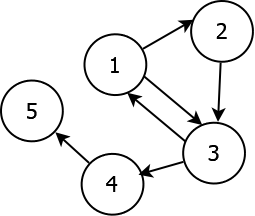
\includegraphics[height=100 pt, width=110 pt]{./ressources/image/graphAdjace.png} 
		\caption{Graphe orienté G}
		\label{grapAdjac}
	\end{center}
	\end{minipage} 
	\begin{minipage}[c]{.46\linewidth}
	\begin{center}
		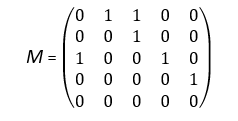
\includegraphics[height=110 pt, width=140 pt]{./ressources/image/matriceAdjac.png} 
		\caption{Matrice d'adjacence du graphe G}
		\label{matriceAdjac}
	\end{center}
	\end{minipage} 
\end{figure} 

\textbf{Place occupée en mémoire :} ${n}^{2}$ pour un graphe d'ordre $|n|$ \citep{lopez2003cours}.			
			\subsection{Matrice d'incidence}
			La matrice d'incidence d'un graphe orienté  G est une matrice de taille $n \times m$  dont les lignes représentent les identifiants des sommets (i $\in$ V) et les colonnes représentent les identifiants des arcs (j $\in$ E) et dont les coefficients (${m}_{ij}$) sont dans \{-1, 0, 1\}, tel que \citep{hennecart2012elements} \citep{mathieu} :
			\[{m}_{ij} :=
			\left\{
			\begin{array}{r c l}
			1 & si $ le sommet i est l'extrémité final de 					l'arc j $ \\
			
			-1 & si $ le sommets i est l'extrémité initial de 				l'arc j $ \\
			0 & sinon \\
			\end{array}
			\right.
			\]
			\\
Pour un graphe non orienté, les coefficients (${m}_{ij}$) de la matrice sont dans \{0, 1\}, tel que \citep{hennecart2012elements} :
			\[{m}_{ij} :=
			\left\{
			\begin{array}{r c l}
			1 & si $ le sommet i est une extrémité					de l'arête j $ \\
			0 & sinon \\
			\end{array}
			\right.
			\]
			\\
\textbf{Exemple :} La figure \ref{matriceIncid} représente 					un exemple d'une matrice d'incidence pour le graphe G ci-contre 			(figure \ref{grapIncid}) :
			
\begin{figure}[H]
	\begin{minipage}[c]{.46\linewidth}
	\begin{center}
		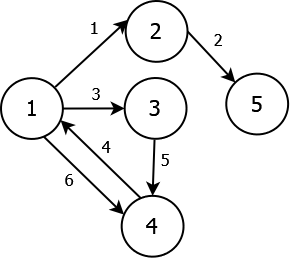
\includegraphics[height=100 pt, width=110 pt]{./ressources/image/graphIncid.png} 
		\caption{Graphe orienté G}
		\label{grapIncid}
	\end{center}
	\end{minipage} 
	\begin{minipage}[c]{.46\linewidth}
	\begin{center}
		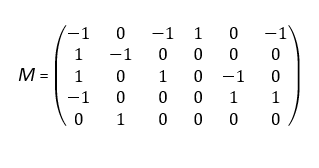
\includegraphics[height=110 pt, width=140 pt]{./ressources/image/matriceIncid.png} 
		\caption{Matrice d'incidence du graphe G}
		\label{matriceIncid}
	\end{center}
	\end{minipage} 
\end{figure}

\textbf{Place occupée en mémoire :} $n \times m$
		
		\subsection{Liste d'adjacence}
			La liste d'adjacence d'un graphe G est un tableau de $|n|$ listes, où chaque entrée (i) du tableau correspond à un sommet et comporte la liste T[i] des successeurs (ou prédécesseurs) de ce sommet, c'est à dire tous les sommets j tel que (i,j) $\in$ E \citep{mathieu}.\\
Dans le cas d'un graphe non orienté, on aura : j $\in$ la liste T[i]  $\iff$ i $\in$ la liste T[j] \citep{IUTLyonInformatique}.

\textbf{Exemple :} La figure \ref{listeAdjac} représente 					un exemple d'une liste d'adjacence pour le graphe G ci-contre 			(figure \ref{grapAdjac2}) :
			
\begin{figure}[H]
	\begin{minipage}[c]{.46\linewidth}
	\begin{center}
		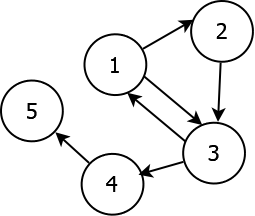
\includegraphics[height=100 pt, width=110 pt]{./ressources/image/graphAdjace.png} 
		\caption{Graphe orienté G}
		\label{grapAdjac2}
	\end{center}
	\end{minipage} 
	\begin{minipage}[c]{.46\linewidth}
	\begin{center}
		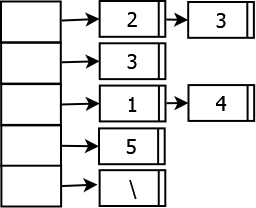
\includegraphics[height=110 pt, width=140 pt]{./ressources/image/listeAdjace.png} 
		\caption{Liste d'adjacence du graphe G}
		\label{listeAdjac}
	\end{center}
	\end{minipage} 
\end{figure}


\textbf{Place occupée en mémoire :} Dans le cas d'un graphe orienté, l'espace occupé par le graphe est de n + m. Dans le cas d'un graphe non orienté, l'espace est de n + 2m car une arête est représentée deux fois.